\documentclass{svproc}
\usepackage{graphicx,amsmath,amssymb,booktabs,url,float}
\usepackage[T1]{fontenc}
\usepackage[utf8]{inputenc}
\usepackage{newtxtext,newtxmath}
\usepackage[hidelinks]{hyperref}
\graphicspath{{../../figures/v2/}}
\newcommand{\AccDirect}{56.7\%}
\newcommand{\AccGraph}{56.1\%}
\newcommand{\AccSingle}{77.8\%}
\newcommand{\AccAlt}{77.8\%}
\newcommand{\AppNodes}{6}
\newcommand{\AppModels}{1}
\newcommand{\RunElapsedHours}{6.91}
\newcommand{\RunGPUHours}{1.94}
\newcommand{\RunResidentHours}{6.12}
\newcommand{\RunOutputTokens}{742,199}
\newcommand{\RunRequests}{1,091}
\newcommand{\RunRequestErrors}{6}
\newcommand{\RunPeakMemory}{22,345}

\begin{document}
\mainmatter
\title{Evidence-Grounded Structural Programs: Assumption-Sensitive Explanations of Joint Causal Pathways}
\titlerunning{Evidence-Grounded Structural Programs}
\author{Anonymous research draft}
\authorrunning{Anonymous}
\institute{Author information withheld}
\maketitle
\begin{abstract}
Narrative evidence can establish an event, support a causal influence, and still fail to identify a structural function. We study whether generative AI can synthesize executable models that expose this distinction and support useful explanations of individual and combined pathways. A local language model proposes operational variables, dependencies, typed mechanisms, alternative interpretations, and prose. Deterministic software validates the expressions, freezes mechanisms and background inputs during interventions, enumerates bounded compatible families, and computes a shared-edge path-coalition allocation. Evidence support remains separate from structural influence. Our frozen controlled evaluation uses 120 independently generated structural causal models, including 72 held-out models, explicit rule texts, intermediate and outcome omissions, and both outcome-changing and outcome-preserving interventions. Direct, graph-conditioned, single-model, and alternative-mechanism methods obtain identified-intervention accuracies of \AccDirect, \AccGraph, \AccSingle, and \AccAlt, respectively. Failed synthesis remains in these denominators. A conditional refinement of an earlier LLM-generated Game of Thrones proposal produces \AppNodes\ retained variables and \AppModels\ functionally distinct models; fresh discovery fails, and its retained causal judgments lack source support. Separate tests assess uncertainty, function agreement, source priority, and explanation/reviewer failures. The study identifies which components execute reliably and which conclusions depend on unverified narrative assumptions. It does not treat controlled counterfactuals as literary validation, generation frequencies as posterior probabilities, or software checks as independent scientific adjudication.
\keywords{structural causal models, program synthesis, narrative evidence, mechanism uncertainty, path attribution}
\end{abstract}

\section{Research question and scope}
Can generative AI synthesize evidence-grounded structural models that support useful, assumption-sensitive explanations of individual and combined causal pathways? A directed graph alone cannot answer this question: an intervention needs a mechanism, and two mechanisms with the same graph and factual state can imply different consequences. A passage can support a directional influence without establishing that a cause is necessary, sufficient, substitutable, or inhibitory.

We evaluate an integration of document-grounded concept discovery, restricted structural-program synthesis, compatible-mechanism execution, and an explicit path-coalition explanation. These components are assessed separately. We do not claim that structural causal models, program synthesis, partial identification, or Shapley allocation are individually novel. The contribution is a specified workflow, its controlled comparisons, and the documented limits of its narrative application.

An earlier prototype is preserved as version 1. Its incomplete benchmark omitted only the outcome rule and contained no identified outcome-changing structural questions in that condition. Its application games were unanimity games, all weakest-link path supports were zero, and its prose and review stages failed. Version 2 changes the scientific protocol rather than silently replacing those results. The old and new benchmarks are different experiments; their aggregate scores are not a paired improvement estimate.

\section{Related work}
Sequence-driven structural causal models use language models as mechanisms within user-defined structures~\cite{bynum}. Here, the LLM proposes variables and dependencies as well as bounded executable mechanisms. LLM-SR studies equation discovery through language-model-guided programming~\cite{shojaee}; sparse narrative observations usually cannot select a unique equation. Narrative graph generation~\cite{li} and event reasoning~\cite{koupaee} supply relevant extraction precedents, while reported tensions between world knowledge and source-specific reasoning motivate source-bounded generation~\cite{yamin}. Shadow-Loom's typed narrative world models provide a close integration precedent~\cite{wilmot}; we make no broad claim to originate executable narrative modeling.

Shapley Flow~\cite{wang}, do-Shapley~\cite{jung,witter}, and PWSHAP~\cite{terminassian} connect attribution with graphs or interventions. Our specified players are paths whose shared edges activate through set union. This game is not asserted to equal those methods, an individual event effect, or a natural path-specific causal effect. Its reference inputs and selected path collection are part of the estimand.

\section{Method}
\subsection{Three evidence judgments}
A variable record contains an operational definition, domain, actor, event and statement times, factual state, explicit reference meaning, source identifiers, and a fact/report/belief distinction. An influence record separately contains endpoint support, directional evidence, contradictions, temporal and information-availability constraints, exact-function assumptions, provenance, and unresolved questions. A character's statement can establish that a claim was made without establishing its content.

The provisional directional weight is 1 for explicit support, 0.5 for contextually supported influence, and 0 otherwise. Unsupported endpoints, missing references, contradictions, or unresolved temporal/information constraints force zero. The exact function's identification status is separate. Unknown functional form therefore does not automatically erase supported direction, and unknown direction is never relabeled to obtain a nonzero ranking. These weights are an explicit heuristic rubric, not causal probabilities or calibrated confidence. Contextual self-review remains dependent on the generating model.

\subsection{Generated and inspectable structural mechanisms}
For a source packet $\mathcal D$ and specified outcome $W$, the LLM proposes variables and mechanisms
\begin{equation}
X_i=f_i(X_{\mathrm{Pa}(i)},U_i).
\end{equation}
The researcher specifies the outcome and documentary scope, not its causes. In the application, source-chunk extraction precedes hierarchical concept selection, individual variable operationalization, LLM-generated admissible ordering, target-centered dependency synthesis, local mechanism proposals, and contextual audits. Context selection prioritizes cited passages, then distinct query-term overlap, with stable ties and declared character budgets. It does not weight term rarity or document length; no retrieval ablation isolates its role in failure. The order excludes cycles but supplies no causal edge. A bounded representation revision receives the actual rejected-mechanism audit and its relevant passages; that audit is itself fallible. Fresh construction requests all concepts, parent choices, expressions, substantive revisions, and explanations from the supplied evidence. The separately labeled fallback initializes from an earlier LLM-generated representation and regenerates operational states and functions; it cannot establish successful fresh discovery. No story mechanism is supplied by the researcher or filled from model memory.

Functions are restricted typed expression trees with explicit parent and background leaves. Validation checks domains, graph/expression agreement, active dependence, acyclicity, applicable time constraints, and reproduction of declared factual states. Arbitrary code execution is unavailable. A parentless variable is an LLM-declared scope boundary. Software serializes that declaration as its external identity input; it is not an inferred upstream story mechanism. Nonroot background inputs require an operational definition, source reference, and substantive justification; an unrestricted residual inserted solely to force factual fit is rejected.

In the application, Boolean/categorical mechanisms with at most 64 input rows are generated as complete LLM-selected output tables, then compiled losslessly into typed expressions. The LLM may request a source-defined background factor through a separate expression proposal; larger domains also use direct expressions. The controlled benchmark retains its separately specified AST synthesis and repair protocol. In the application, the LLM may explicitly retract a provisional parent with a source-based reason. Software certifies invariance across the entire generated finite table and still requires every retained parent to be active. Retractions precede outcome computation, preserve aligned node meanings, and remain visible in the audit. A resulting parentless constant is a declared observed scope boundary with unexplained upstream causes, not an added residual; losing all outcome ancestry is a construction failure. Small discrete functions receive exhaustive truth tables. Larger domains receive declared bounded probes. Reports expose where changing a parent changes the child, necessary and sufficient input conditions, joint enabling, substitution, inhibitory or mixed polarity, and remaining untested behavior. Authoritative descriptions are derived from actual behavior; the original generated description is retained for audit. A conjunction cannot be described as making either conjunct sufficient. Mathematical consistency does not show that a narrative obeys that function.

For $\mathrm{do}(X_A=a)$, only the targeted equations are replaced. All other mechanisms remain fixed, and the factual background $u^*$ is reused in factual and counterfactual worlds. Structural assumptions are never regenerated during execution.

\subsection{Compatible alternatives}
When text leaves a function unresolved, the controlled solver considers all active deterministic Boolean functions of the declared inputs compatible with the observed row. Multiple omitted functions are enumerated jointly. The implementation also supports bounded candidate families for larger finite inputs, with explicit limits of 256 local tables and 512 combined candidates. Every result states whether coverage is exhaustive within its declared family or sampled/bounded. Omitted variables, alternative graphs, and arbitrary confounding lie outside this guarantee.

Application alternatives are generated and screened against contextual evidence and actual function behavior. Functionally identical candidates are deduplicated. The retained global set has at most 12 models: a principal model, bounded local changes across the graph, and bounded joint changes chosen before computing outcomes or allocations; it is not an exhaustive Cartesian family. An unresolved compatibility judgment remains unresolved. For aligned interventions, we report outcome sets across retained models, not probabilities inferred from their generation frequency. A single interpretation cannot establish robustness across interpretations.

\subsection{Shared-edge path coalition}
Let $\mathcal P$ be a recorded, source-balanced, shortest-first selection of at most eight paths to $W$. For coalition $S\subseteq\mathcal P$, let $E(S)=\bigcup_{p\in S}E(p)$ and $E_F=\bigcup_{p\in\mathcal P}E(p)$. Edges in $E_F\setminus E(S)$ supply declared reference parent inputs; edges outside $E_F$ remain active. In fixed background $u^*$,
\begin{equation}
v(S)=W_{M_{E(S)}}(u^*),\qquad
\phi_p=\sum_{S\subseteq\mathcal P\setminus\{p\}}
\frac{|S|!(|\mathcal P|-|S|-1)!}{|\mathcal P|!}
\bigl[v(S\cup\{p\})-v(S)\bigr].
\end{equation}
Shared edges execute once. Exact enumeration accounts for overlap, interactions, redundancy, and negative game contributions, and satisfies $\sum_p\phi_p=v(\mathcal P)-v(\varnothing)$. Edge unions can enable recombined routes. The selected-edge contrast need not equal the entire effect of an event intervention if paths are omitted. Signs describe the chosen contrast; removing a positively influential event can yield a negative allocation without making that event intrinsically inhibitory.

We report the distribution of all coalition outcomes, unanimity, minimal full-outcome coalitions, substitutes, negative marginals, and pair interactions. Minimality checks every strict subset, including in nonmonotone games. Equal allocations are not altered: both conjunction and redundancy can produce equal shares while implying different coalition behavior. Reference and path-set sensitivity are essential. Paths are compared across models only when their meanings and node sequences align.

For path $p$, let $c_p=\min_{e\in p}c_e$. Supporting source clusters divide a unit allocation $a_{\ell p}$, and segment priority is
\begin{equation}
R_\ell=\sum_p a_{\ell p}c_p|\phi_p|.
\end{equation}
Evidence weights do not enter the structural equations. High-influence, weak-evidence paths remain visible separately. If all priorities are zero, the ranking is unavailable. The priority is not the causal effect of deleting text, and a zero modeled contrast can leave important evidence for invariance unranked.

\subsection{Explanation and review}
Software first assembles the exact intervention, factual and counterfactual states, possible outcomes, paths, signed allocations, ties, evidence references, and assumptions. The LLM explains supplied numbers without recalculating them. Actual prose is split into fixed sentence IDs before review. Software rejects unknown identifiers, disallowed numeric claims, simple explicit outcome-value mismatches, and unqualified uniqueness among ties. Source identifiers remain in the structured record without presenting internal allocation weights as story quantities. The semantic reviewer evaluates those exact IDs against the computed record and supplied source context; nonexistent sentence IDs or quoted audit instructions are invalid reviews.

Explanation failure and reviewer failure are recorded separately. Known review controls contain a true factual value, a flipped factual value, an invalid probability interpretation, and a statement of dependence on equations and references. Their expected labels are withheld. These controls test limited trace interpretation, not independent literary entailment. A compact source/equation review packet is prepared for the researcher; no human adjudication is inferred from its existence.

\section{Frozen evaluation}
The generator creates 120 independent SCMs, split into 24 development, 24 calibration, and 72 test models. Sizes are eight and twelve variables, with conjunction, redundancy, exclusive interaction, inhibition, shared causes, and reconverging routes. The four balanced conditions are complete rules, missing intermediate rules, a missing outcome rule, and two missing rules. The generating program, omissions, factual inputs, and questions are fixed without inspecting method outputs. Each generating SCM stays within one split; no uncontrolled paraphrases are added. All 120 visible narratives are distinct.

Texts explicitly state available rules and observed states. Each SCM receives all non-outcome single flips, three seeded joint flips, and three factual-value controls. No question directly overrides the outcome. The test set has 1,080 questions: 129 identified changes, 729 identified preservations, and 222 underidentified queries. Complete outcome-rule omission with only a factual-row constraint cannot identify a changed outcome in this declared family; changed identified incomplete queries instead occur in the intermediate and multiple-omission conditions. Both factual outcome states occur.

B0 answers directly from the record. B1 receives the identical record plus generated adjacency, without equations. A usable graph may survive expression failure. B2 executes one accepted synthesized model. ALT executes the declared compatible family. FULL shares ALT's outcome sets and adds paths, evidence priorities, and reviewed prose; its additional components are not credited through ALT's answer score. CARRY retains the factual outcome. ORACLE\_FAMILY receives the compatible family and provides an information ceiling; ORACLE\_TRUE receives the hidden generating program and provides a point-prediction diagnostic with extra information.

Synthesis permits at most two repairs: one local expression replacement and then one fresh reconstruction, using original text and candidate factual-row diagnostics only. Hidden generating equations and gold query answers never enter prompts or repair feedback. The retained development trials document unsuccessful constant, expression, and finite-table repairs. One final pilot SCM still fails synthesis; rejection is preserved, not counted as an accepted end-to-end example. The technical gate checks distinct information configurations, valid-model numerical reproduction, sentence review, and actual-host process supervision. The application reaches this technical gate only through conditional refinement and a retained-response literal syntax recovery; fresh discovery and application prose remain failed components. The controlled benchmark retains its original AST interface, so its scores do not validate the different application synthesis interface.

Primary estimates average within SCM before averaging across independent SCMs. All planned test SCMs, including failed synthesis, remain in relevant denominators. A stratum with no eligible questions in an SCM is omitted only for that stratum. We use 5,000 paired SCM bootstrap resamples with fixed seed 271828 and descriptive percentile intervals. Successful-synthesis-only results are secondary. Calibration records are kept separate; no calibrated probability claim is made. No experiment is extended to seek statistical significance.

Known nonroot functions are compared over all Boolean parent inputs. Controlled grounding checks factual states, declared directions, and source-rule references. Source nDCG@5 uses an independently specified gold affected-mechanism slice, with higher relevance for explicit rules than missing-rule statements. Unaffected background evidence is outside these positive labels; they are not human literary relevance judgments or minimal sufficient evidence sets. Factual-value controls may be resolved from observed states and intervention semantics despite positive downstream slice labels. The corpus does not independently manipulate source reliability, limiting claims about the benefit of evidence weighting. Missing rankings score zero where positive labels exist. Runtime, tokens, and failure rates are reported separately.

\section{Measured component results}
All 72 planned held-out SCM records completed. Table~\ref{tab:primary} reports SCM means with descriptive 95\% bootstrap intervals. Failed synthesis remains in each relevant primary denominator. FULL and ALT have identical outcome answers by construction; the additional FULL components are assessed separately.

Eligible independent SCM counts are 72 for identified questions, 40 for outcome changes, 72 for preserved outcomes and 51 for underidentified questions. Eligibility follows the fixed questions, never method success.

\begin{table}[t]\centering\small\setlength{\tabcolsep}{3pt}

\caption{Identified and underidentified questions; estimates and 95\% intervals.}\label{tab:primary}

\begin{tabular}{lrrrr}\toprule Method & Identified & Changes & Preserves & Uncertainty\\\midrule

B0 & \shortstack{0.567\\{[0.478, 0.658]}} & \shortstack{0.546\\{[0.410, 0.678]}} & \shortstack{0.569\\{[0.473, 0.668]}} & \shortstack{0.431\\{[0.304, 0.569]}}\\

B1 & \shortstack{0.561\\{[0.474, 0.647]}} & \shortstack{0.567\\{[0.436, 0.695]}} & \shortstack{0.569\\{[0.478, 0.661]}} & \shortstack{0.377\\{[0.245, 0.510]}}\\

B2 & \shortstack{0.778\\{[0.681, 0.875]}} & \shortstack{0.800\\{[0.675, 0.925]}} & \shortstack{0.778\\{[0.681, 0.875]}} & \shortstack{0.000\\{[0.000, 0.000]}}\\

ALT & \shortstack{0.778\\{[0.681, 0.875]}} & \shortstack{0.800\\{[0.675, 0.925]}} & \shortstack{0.778\\{[0.681, 0.875]}} & \shortstack{0.529\\{[0.392, 0.667]}}\\

CARRY & \shortstack{0.862\\{[0.820, 0.902]}} & \shortstack{0.000\\{[0.000, 0.000]}} & \shortstack{1.000\\{[1.000, 1.000]}} & \shortstack{0.000\\{[0.000, 0.000]}}\\

ORACLE\_FAMILY & \shortstack{1.000\\{[1.000, 1.000]}} & \shortstack{1.000\\{[1.000, 1.000]}} & \shortstack{1.000\\{[1.000, 1.000]}} & \shortstack{1.000\\{[1.000, 1.000]}}\\

\bottomrule\end{tabular}\end{table}

\begin{table}[t]\centering\small\setlength{\tabcolsep}{3pt}

\caption{Complete versus incomplete mechanisms. Changed and preserved strata are scored separately.}\label{tab:missing}

\begin{tabular}{llrrr}\toprule Condition & Method & Changes & Preserves & Uncertainty\\\midrule

complete & B0 & \shortstack{0.666\\{[0.489, 0.831]}} & \shortstack{0.724\\{[0.574, 0.862]}} & ---\\

complete & B2 & \shortstack{1.000\\{[1.000, 1.000]}} & \shortstack{1.000\\{[1.000, 1.000]}} & ---\\

complete & ALT & \shortstack{1.000\\{[1.000, 1.000]}} & \shortstack{1.000\\{[1.000, 1.000]}} & ---\\

omit intermediate & B0 & \shortstack{0.567\\{[0.327, 0.793]}} & \shortstack{0.696\\{[0.542, 0.830]}} & \shortstack{0.133\\{[0.000, 0.300]}}\\

omit intermediate & B2 & \shortstack{0.600\\{[0.333, 0.867]}} & \shortstack{0.667\\{[0.444, 0.889]}} & \shortstack{0.000\\{[0.000, 0.000]}}\\

omit intermediate & ALT & \shortstack{0.600\\{[0.333, 0.867]}} & \shortstack{0.667\\{[0.444, 0.889]}} & \shortstack{0.467\\{[0.200, 0.733]}}\\

omit outcome & B0 & --- & \shortstack{0.456\\{[0.235, 0.678]}} & \shortstack{0.556\\{[0.333, 0.778]}}\\

omit outcome & B2 & --- & \shortstack{1.000\\{[1.000, 1.000]}} & \shortstack{0.000\\{[0.000, 0.000]}}\\

omit outcome & ALT & --- & \shortstack{1.000\\{[1.000, 1.000]}} & \shortstack{0.722\\{[0.500, 0.889]}}\\

multiple missing & B0 & \shortstack{0.190\\{[0.000, 0.476]}} & \shortstack{0.397\\{[0.207, 0.604]}} & \shortstack{0.556\\{[0.333, 0.778]}}\\

multiple missing & B2 & \shortstack{0.714\\{[0.429, 1.000]}} & \shortstack{0.444\\{[0.222, 0.667]}} & \shortstack{0.000\\{[0.000, 0.000]}}\\

multiple missing & ALT & \shortstack{0.714\\{[0.429, 1.000]}} & \shortstack{0.444\\{[0.222, 0.667]}} & \shortstack{0.389\\{[0.167, 0.611]}}\\

\bottomrule\end{tabular}\end{table}

\paragraph{Paired comparisons.}

B1 minus B0: identified accuracy -0.007 [-0.055, 0.046]; outcome-changing accuracy 0.021 [-0.085, 0.135]; appropriate uncertainty -0.054 [-0.147, 0.034].

B2 minus B0: identified accuracy 0.210 [0.096, 0.328]; outcome-changing accuracy 0.254 [0.088, 0.420]; appropriate uncertainty -0.431 [-0.569, -0.304].

ALT minus B2: identified accuracy 0.000 [0.000, 0.000]; outcome-changing accuracy 0.000 [0.000, 0.000]; appropriate uncertainty 0.529 [0.392, 0.667].

FULL minus B0: identified accuracy 0.210 [0.096, 0.328]; outcome-changing accuracy 0.254 [0.088, 0.420]; appropriate uncertainty 0.098 [-0.108, 0.294].

FULL minus CARRY: identified accuracy -0.085 [-0.191, 0.016]; outcome-changing accuracy 0.800 [0.675, 0.925]; appropriate uncertainty 0.529 [0.392, 0.667].

\paragraph{Separate synthesis, grounding, and explanation components.}

\begin{table}[t]\centering\small\begin{tabular}{lr}\toprule Component & Estimate [95\% interval]\\\midrule

synthesis first & 0.444 [0.333, 0.556]\\

synthesis after repair & 0.778 [0.681, 0.875]\\

known function agreement & 0.778 [0.681, 0.875]\\

unknown flag accuracy & 0.764 [0.667, 0.856]\\

direction precision & 0.778 [0.681, 0.875]\\

direction recall & 0.778 [0.681, 0.875]\\

direction grounding & 0.778 [0.681, 0.875]\\

event state agreement & 0.778 [0.681, 0.875]\\

explanation generated & 0.778 [0.681, 0.875]\\

explanation deterministic pass & 0.569 [0.458, 0.681]\\

reviewer valid ids & 0.778 [0.681, 0.875]\\

explanation same model supported & 0.681 [0.569, 0.778]\\

explanation displayable & 0.556 [0.444, 0.667]\\

reviewer control accuracy & 0.698 [0.608, 0.788]\\

reviewer control false acceptance & 0.021 [0.000, 0.049]\\

reviewer control missing & 0.222 [0.125, 0.319]\\

\bottomrule\end{tabular}\caption{Components use all planned test SCMs. Same-model semantic review is dependent.}\label{tab:components}\end{table}

\paragraph{Source prioritization.}

B0 nDCG@5: 0.658 [0.538, 0.771].

B1 nDCG@5: 0.722 [0.610, 0.825].

FULL nDCG@5: 0.417 [0.260, 0.568].

UNIFORM nDCG@5: 0.417 [0.260, 0.568].

Paired FULL minus B0: -0.241 [-0.433, -0.050].

Paired FULL minus B1: -0.305 [-0.485, -0.119].

Paired FULL minus UNIFORM: 0.000 [0.000, 0.000].

The independently fixed relevance labels describe the affected-mechanism slice, not human reading value. A zero modeled contrast can yield no ranking even when passages help explain invariance. The uniform-support ablation shares the same paths and allocations. Full results, conditional successful-synthesis estimates, error records, and all completeness strata accompany the release.

\paragraph{Held-out computation.}

The 469 held-out requests used 346,333 response-reported output tokens, identified by exact narrative matching. Summed request durations are 2.53 hours and overlap across workers; they are not elapsed GPU time. Synthesis requests are shared by B1, B2, ALT and FULL. The release separates incremental costs by request role, including prose generation, review and controls.

\begin{figure}[t]\centering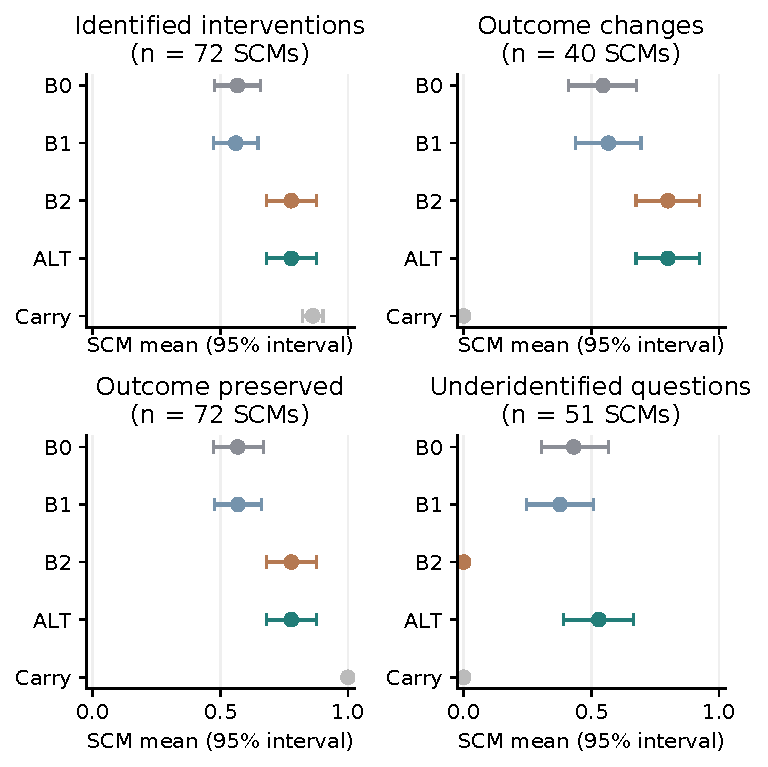
\includegraphics[width=\linewidth]{benchmark_components.pdf}\caption{Held-out SCM means and 95\% paired-unit bootstrap intervals.}\label{fig:benchmark}\end{figure}

\section{Narrative application and audits}
Armed conflict between the Stark-led northern/Riverlands coalition and the Lannister-controlled crown is active by the end of season 1. We acquired ten first-season episode transcriptions from ScreenScripts~\cite{screenscripts}. They are traceable documentary material, not authenticated official scripts; transcription fidelity and interpretation require researcher review.

Variables and dependencies initialize from an earlier LLM-generated proposal. Operational states/references are regenerated against the new transcript context, all nonroot mechanisms are newly proposed, and dependency retractions remain possible. This is conditional refinement, not successful fresh variable/dependency discovery.

The LLM retained 6 variables and 7 directed influences. This application has one functional hypothesis, one intervention-outcome vector and one retained local-option combination. There is no demonstrated agreement across alternatives, and singleton outcome sets are consequences of that hypothesis, not identification from the sources.

Four retained variables are fixed scope boundaries with unexplained upstream causes; only two functions connect endogenous variables. The ten-node target was not met. All seven directional judgments are unsupported. Targeted assistant inspection additionally flags planned versus realized actions, event timing, an inconsistent outcome audit, and reference-policy ambiguity. These are unresolved review issues, not independently adjudicated error labels.

The six-path game has 59 coalitions with outcome zero and 5 with outcome one. Two minimal full-outcome coalitions provide substitute routes, so the full set of six paths is unnecessary. It has 1 negative coalition marginal; its pair-interaction range is [-1, 1], exposing both joint enabling and substitution within the assumed program.

Table~\ref{tab:applicationpaths} identifies the selected paths and their signed allocations. Evidence-weighted source ranking was unavailable because all scores were zero. No unsupported score was raised to create an ordering.

\begin{table}[t]\centering\small\setlength{\tabcolsep}{5pt}
\caption{The six-path global game. Node IDs map to the event labels in Fig.~\ref{fig:flagship}; $c_p$ is weakest directional support.}\label{tab:applicationpaths}
\begin{tabular}{llrr}\toprule Path & Node sequence & $\phi_p$ & $c_p$\\\midrule
p1 & \texttt{X03} $\to$ \texttt{W} & $0.26667$ & 0.0\\
p2 & \texttt{X06} $\to$ \texttt{W} & $0.26667$ & 0.0\\
p3 & \texttt{X07} $\to$ \texttt{X09} $\to$ \texttt{W} & $-0.03333$ & 0.0\\
p4 & \texttt{X08} $\to$ \texttt{W} & $0.26667$ & 0.0\\
p5 & \texttt{X06} $\to$ \texttt{X09} $\to$ \texttt{W} & $0.21667$ & 0.0\\
p6 & \texttt{X08} $\to$ \texttt{X09} $\to$ \texttt{W} & $0.01667$ & 0.0\\
\bottomrule\end{tabular}\end{table}

The application explanation failed the displayability checks. It contains six actual sentences instead of at most four and cites nonexistent numerical field names. The reviewer covers all six actual IDs but labels their text supported. Its controls score three of four: the probability claim is marked unverifiable rather than unsupported, with no false acceptance. Valid sentence coverage does not establish narrative entailment.

Both factual-null and domain-endpoint reference checks yield zero allocations. Here their seven edge-reference assignments are identical: they are one null contrast, not two distinct robustness scenarios or defensible alternative histories. A four-path collection is a unanimity game: fifteen coalitions yield zero and one yields one, with four equal one-quarter shares. For the aligned scout-to-capture-to-war path, changing from six to four players changes its share from minus one-thirtieth to one-quarter without changing any equation. In the four-path game, mobilization-to-capture remains outside the selected union and active; the scout path bundles the necessary capture-to-outcome edge. Its positive allocation is therefore not an individual effect of the scout action. The factual intervention removing that action instead leaves the outcome unchanged. None of these quantities is a probability or historical responsibility.

The source/equation audit, full-context private review packet, and blank independent review form remain available. These artifacts do not imply completed human adjudication. Local function behavior and shared outcome queries are reported separately; unresolved source compatibility remains a hypothesis.

\begin{figure}[p]\centering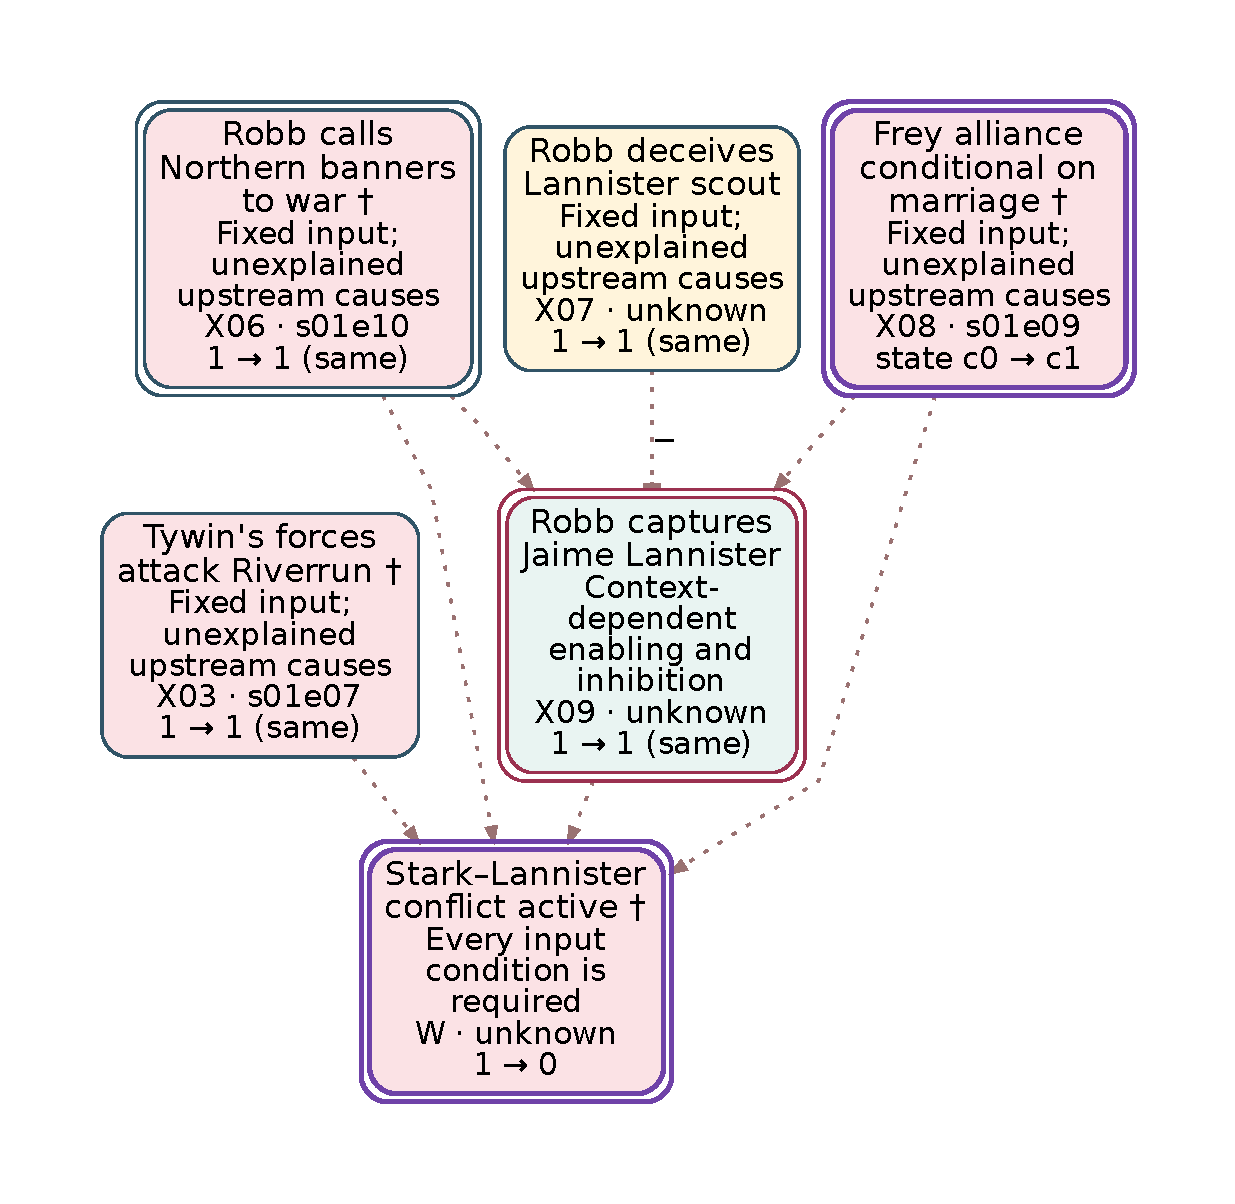
\includegraphics[width=\linewidth,height=.86\textheight,keepaspectratio]{five_kings_network.pdf}\caption{Conditional hypothesis, not an established causal account. States show one frozen-mechanism intervention: violet borders change, double borders mark shared pathways, and dotted edges have zero directional support. A tee marks a modeled inhibitory effect; daggers flag operational/source concerns. Four nodes are unexplained scope boundaries. Category c0 allows passage conditional on marriage; c1 refuses it without an agreement, an unresolved reference interpretation.}\label{fig:flagship}\end{figure}
\begin{figure}[t]\centering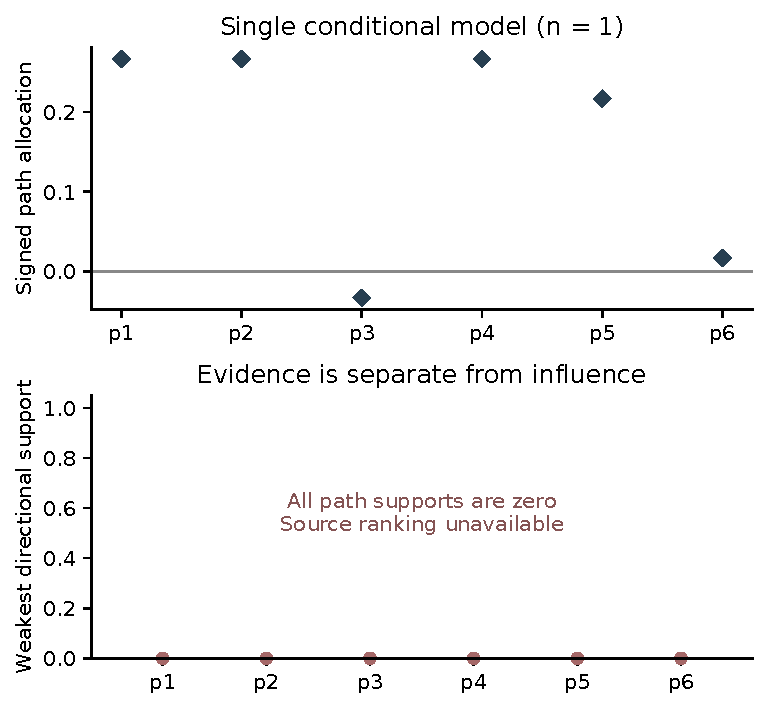
\includegraphics[width=\linewidth]{path_influence_evidence.pdf}\caption{Six-path coalition allocations for one conditional model; directional support is separately zero. These shares explain the declared coalition contrast, not the particular event intervention annotated in Fig.~\ref{fig:flagship}.}\label{fig:path}\end{figure}
\begin{figure}[t]\centering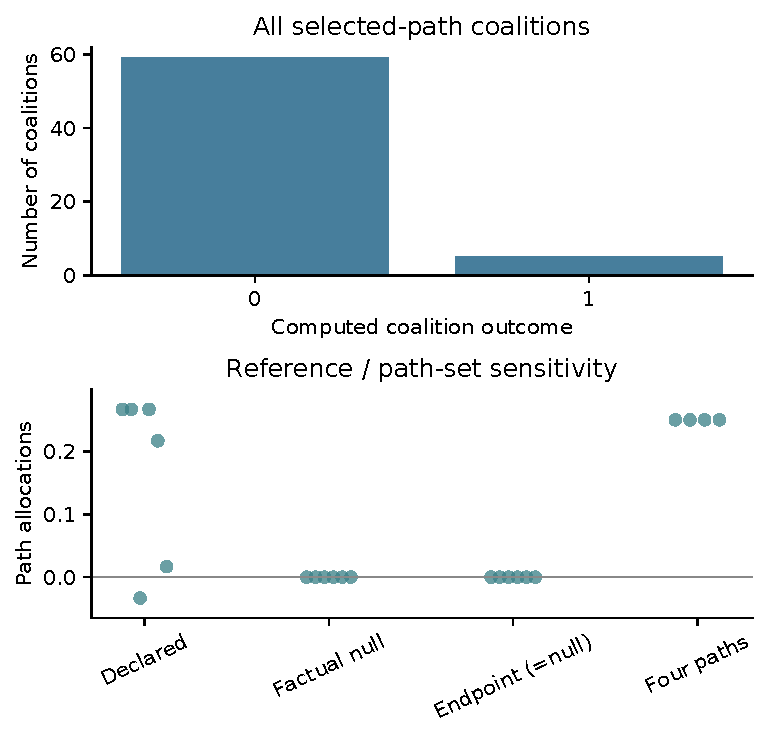
\includegraphics[width=\linewidth]{coalition_sensitivity.pdf}\caption{Coalition outcomes and sensitivity to references and selected paths. Dots represent individual path allocations, with horizontal offsets exposing ties. The four-path collection defines a different coalition game.}\label{fig:sensitivity}\end{figure}

\section{Limitations and scientific decision}
The controlled comparisons concern extraction and execution of explicit rule records. They do not establish open-ended concept discovery or a grounded literary explanation. Differences between version 1 and version 2 aggregate scores are not paired evidence of improvement: the generating SCMs, omissions, questions, and scoring targets changed. Only the within-version paired comparisons support component comparisons.

Those comparisons support executing a synthesized program for identified queries in this controlled setting. B2 gains 0.210 [0.096, 0.328] over direct answers overall and 0.254 [0.088, 0.420] on changed-outcome questions. A generated graph alone shows no clear gain. Every admitted test model reproduces the known functions, declared directions and factual states exactly, but 16 of 72 syntheses fail. The first attempt succeeds on 32 models; bounded repairs recover 24 more. Complete and missing-outcome conditions each admit all 18 models, whereas intermediate and multiple omissions admit 12 and eight. The primary scores expose that bottleneck rather than reporting only conditional perfection.

Alternative execution improves appropriate uncertainty over the necessarily point-valued B2 answers by 0.529 [0.392, 0.667], without changing identified-query accuracy. Its gain over direct answers on uncertainty, 0.098 [$-0.108$, 0.294], remains inconclusive. Nine admitted models fail to mark ten missing rules, yielding families that are too narrow; a correct solver cannot infer a missing uncertainty declaration. CARRY reaches 0.862 identified accuracy by preserving the factual outcome, yet scores zero on outcome changes. The aggregate result therefore cannot replace the changed/preserved decomposition.

The source-priority finding is negative. FULL obtains nDCG@5 of 0.417 versus 0.658 for B0 on 37 eligible SCMs; their paired difference is $-0.241$ [$-0.433$, $-0.050$]. Only 16 of these 37 records have a FULL ranking: ten fail synthesis and eleven admit a model but yield no priority. Uniform support gives identical scores. These labels and this corpus do not demonstrate a benefit from evidence weighting, and priorities from one assumed model need not cover family uncertainty.

Forty of 72 explanations pass the frozen displayability checks. All 56 generated explanations and their control reviews use valid actual sentence IDs, but that contract does not ensure judgment quality. Fifteen controls incorrectly reject a true factual value; three accept its deliberately flipped counterpart. Among performed controls, strict agreement is 201/224, with 3/112 false acceptances on deliberately unsupported statements. These repeated controls are conditional diagnostics, not independent human assessments. For example, record \texttt{v2\_scm\_278011} rejects a true factual value because the counterfactual value differs. This explicitly confuses the worlds that an explanation should distinguish.

The narrative application remains a failure to establish the main grounding objective. Fresh construction did not reach an admissible final model. Conditional refinement produced a single small interpretation with four unexplained scope boundaries, seven unsupported directional influences, and zero weakest-link support for every path. A richer accessible corpus and more inspectable equations were insufficient to produce a defensible source-weighted ranking. Neither formal admission nor a completed figure converts that hypothesis into a supported account of the conflict.

Protocol restrictions also require scrutiny. An LLM-generated order, at most four direct parents, bounded passage context, outcome-ancestor pruning, and local finite tables constrain the search. Requiring every retained parent to be active can reject a proposed representation; allowing source-reasoned retraction then reduced this case to four fixed boundaries and two connected functions. The protocol permits justified background factors, but this retained model has none. No ablation separates these constraints from model capability or variable-definition errors. The small graph is therefore not evidence that the conflict has only these causes, and broader function coverage cannot repair missing concepts or unsupported directions.

The coalition analysis supplies useful distinctions about an assumed program: it separates unanimity from substitutable routes, exposes inhibitory coalition contexts, and reveals player-selection sensitivity. A sign change under path selection, together with a zero individual event effect, shows why a bundled-path share must not be described as an event's historical responsibility. The endpoint and factual-null policies coincide in this application, so their identical zero allocations provide a single null-contrast check, not robustness across distinct plausible histories. These are mathematical distinctions and limits. Their usefulness for selecting narrative evidence or improving reader understanding remains unestablished.

The manuscript therefore supports a narrower controlled-methods evaluation and failure-analysis contribution, not a validated Game of Thrones application contribution. The complete three-conflict application objective has not been achieved. Northern and Daenerys cases remain preserved version-1 limitations; no new transfer experiment is claimed. A second model, additional application seeds, and a reader study were not run.

Researcher adjudication is required for transcription fidelity, event/report/belief distinctions, timing and information availability, planned versus realized actions, composite operational definitions, and reference meanings. The modeled necessity of tactical outcomes for the conflict and the generated inhibitory assumption also require separate scrutiny. The independent review form remains unfilled. The supplied source passages, equations, behavior tables, and flagged questions make those decisions inspectable without pretending that human review has occurred.

The controlled texts are explicit logical records, not proof of open-domain narrative understanding. A deterministic compatible family conditions on its graph, inputs, domains, and factual observations. Alternative graph structures, missing concepts, latent causes, and uncertain chronology can dominate uncertainty outside that family. Repeated generations or wording changes do not provide independent model diversity.

Application evidence comes from accessible unofficial transcriptions whose fidelity to the aired television continuity requires review. Source access, exact references, and a matching quotation do not establish entailment. Source-bounded prompts cannot certify that pretrained world knowledge played no role; an attached reference alone is not entailment. Same-model generation and audit are dependent, and factual grounding, causal direction, and structural necessity must be adjudicated separately. The review packet is a concrete review aid, not a completed human study.

Path attribution explains a defined model contrast. Player selection, overlap, reference inputs, and unmodeled context can alter the allocation. Equal shares can be valid but uninformative; nonzero source priorities need not identify the best passages for human understanding. No causal probability, reader-comprehension improvement, human-review outcome, or independent literary counterfactual gold is claimed. Passing tests establishes specific implementation properties, not scientific validity.

\section*{Reproducibility and resource limits}
The campaign has a separately persisted 24-hour deadline, a four-hour analysis/delivery reserve, project-scoped process supervision, and periodic local synchronization. It reuses a cached Qwen3-14B-AWQ model on an existing RTX 4090 with 24 GB VRAM. The measured pilot determines a 1.1-million-output-token safety ceiling. No external paid inference, pod creation, billing change, or unrelated-service shutdown is used. Code, frozen configuration, compact records, vector figures, and the anonymous draft form the release; full transcripts, weights, prompts, and raw logs remain local. Version 1 records and its deadline are preserved. The final resource accounting accompanies the numerical results.

\section*{Declaration on Generative AI}
An AI coding assistant implemented and executed the researcher-directed revision, analyzed retained artifacts, and drafted this manuscript. Qwen3-14B-AWQ generated experimental concepts, dependencies, mechanisms, source judgments, revisions, and explanations. Software computed interventions, allocations, and statistical summaries. Human scientific adjudication and final author responsibility remain pending. This is an unsubmitted research draft; AI systems are not authors, and software or same-model review is not represented as human approval.

\clearpage
\begin{thebibliography}{12}
\bibitem{bynum} Lucius E.J. Bynum; Kyunghyun Cho: Language Models as Causal Effect Generators. Proceedings of the 2025 Conference on Empirical Methods in Natural Language Processing, 2025. \url{https://aclanthology.org/2025.emnlp-main.107/}.
\bibitem{shojaee} Shojaee, Parshin; Meidani, Kazem; Gupta, Shashank; Barati Farimani, Amir; Reddy, Chandan: LLM-SR: Scientific Equation Discovery via Programming with Large Language Models. International Conference on Learning Representations, 2025. \url{https://proceedings.iclr.cc/paper_files/paper/2025/hash/28df8e730c054c5331855fd4d5403ba9-Abstract-Conference.html}.
\bibitem{li} Zehan Li; Ruhua Pan; Xinyu Pi: Beyond LLMs A Linguistic Approach to Causal Graph Generation from Narrative Texts. Proceedings of the 7th Workshop on Narrative Understanding, 2025. \url{https://aclanthology.org/2025.wnu-1.10/}.
\bibitem{koupaee} Mahnaz Koupaee; Xueying Bai; Mudan Chen; Greg Durrett; Nathanael Chambers; Niranjan Balasubramanian: Causal Graph based Event Reasoning using Semantic Relation Experts. Proceedings of the 63rd Annual Meeting of the Association for Computational Linguistics (Volume 1: Long Papers), 2025. \url{https://aclanthology.org/2025.acl-long.1269/}.
\bibitem{yamin} Yamin, Khurram; Gupta, Shantanu; Ghosal, Gaurav; Lipton, Zachary; Wilder, Bryan: LLMs Struggle to Balance Reasoning and World Knowledge in Causal Narrative Understanding. International Conference on Learning Representations, 2026. \url{https://proceedings.iclr.cc/paper_files/paper/2026/hash/98741856b327ec2f9503179398da662f-Abstract-Conference.html}.
\bibitem{wilmot} Wilmot, David: Shadow-Loom: Causal Reasoning over Graphical World Models of Narratives. arXiv preprint 2605.02475, 2026. \url{https://arxiv.org/abs/2605.02475}.
\bibitem{wang} Jiaxuan Wang; Jenna Wiens; Scott Lundberg:  Shapley Flow: A Graph-based Approach to Interpreting Model Predictions . International Conference on Artificial Intelligence and Statistics, 2021. \url{https://proceedings.mlr.press/v130/wang21b.html}.
\bibitem{jung} Yonghan Jung; Shiva Kasiviswanathan; Jin Tian; Dominik Janzing; Patrick Bloebaum; Elias Bareinboim: On Measuring Causal Contributions via do-interventions. International Conference on Machine Learning, 2022. \url{https://proceedings.mlr.press/v162/jung22a.html}.
\bibitem{terminassian} Lucile Ter-Minassian; Oscar Clivio; Karla Diazordaz; Robin J. Evans; Christopher C. Holmes: PWSHAP: A Path-Wise Explanation Model for Targeted Variables. International Conference on Machine Learning, 2023. \url{https://proceedings.mlr.press/v202/ter-minassian23a.html}.
\bibitem{witter} R. Teal Witter; Álvaro Parafita; Tomas Garriga; Maximilian Muschalik; Fabian Fumagalli; Axel Brando; Lucas Rosenblatt: Exactly Computing do-Shapley Values. International Conference on Machine Learning, 2026. \url{https://proceedings.mlr.press/v306/witter26a.html}.
\end{thebibliography}
\end{document}
